\documentclass{article}

% set font encoding for PDFLaTeX or XeLaTeX
\usepackage{graphicx}
\usepackage{ifxetex}
\ifxetex
  \usepackage{fontspec}
\else
  \usepackage[T1]{fontenc}
  \usepackage[utf8]{inputenc}
  \usepackage{lmodern}
\fi
\title{Actividad 4}
\author{Corral Valdez Jesus Giovanni\\
Departamento de Física
}

% Enable SageTeX to run SageMath code right inside this LaTeX file.
% documentation: http://mirrors.ctan.org/macros/latex/contrib/sagetex/sagetexpackage.pdf
% \usepackage{sagetex}

\begin{document}
\maketitle
\section{Movimiento de proyectil con fricción del aire}
Cuando se trabaja con movimiento de proyectiles en un fluido, por ejemplo el de una esfera en el aire (considerado un fluido con muy baja densidad), se tienen en cuenta dos conceptos muy importantes: velocidad terminal y coefciente de arrastre. Estos datos se utilizaran para calcular la constante necesaria para los calculos de velocidades y posiciones del movimiento.
\begin{equation}
C=
\end{equation}


\subsection{Coeficiente de arrastre}
El coeficiente de arrastre es una cantidad adimensional que se usa para cuantificar el arrastre o resistencia de un objeto en un medio fluido como el agua o el aire.
Se calcula de la siguiente manera:
\begin{equation}
Cd = 2F_d/pv^2A
\end{equation}
Donde Fd es la fuera de arrastre, p la densidad del fluido, v la rapidez del objeto y A es el area de referencia.

\subsection{Velocidad Terminal}
La velocidad terminal es la velocidad en la que un objeto se mantendra despues de acelerar y desacelerar por la distintas fuerzas, en este caso la fuerza de gravedad y la provocada por el arrastre del fluido. Se calcula de la siguiente manera:
\begin{equation}
v_t=\sqrt{2mg/pAC_d}
\end{equation}

\section{Actividad}
\subsection{Código Fortran}
Se utilizó el siguiente código para desarrollar el programa que da los datos de posición de un lanzamiento de una esfera en distintas velocidades en un angulo de 45 grados.

\begin{verbatim}
program resistencia
  implicit none
  integer :: i, v
  real :: vt
  integer, parameter :: ntimes = 10000
  real, dimension (10000) :: vx,vy
  real, dimension (10000) :: x,y
  real :: time, fa, fi, fv, area, constant
  real, parameter :: deltat = 0.01
  real, parameter :: g = 9.8
  real, parameter :: pi = 3.1415927
  real, parameter :: m = 0.142, d = 0.07, cd = 0.47 !Son, respectivamente, la masa (kg), el diametro (m) y el coeficiente de arrastre de la esfera. 
  real, parameter :: p = 1.225 !densidad del aire en kg/m³.
  real, parameter :: radian = pi / 4 !trabajaremos con 45 grados

  area = d * d * pi
  area = area / 4
  vt = 2 * m * g / (p * area * cd)
  vt = SQRT(vt)
  constant =  m * g / vt
  write (*,*) 'Constante: ',constant ! Estas operaciones son necesarias para encontrar la constante que se utilizara en el calculo de la posición.

  
  open (1, file = 'datos.dat', status = 'unknown')
    do v=10, 100, 10
        fv = float(v)
 
     do  i=1, ntimes  
        fi = float(i)
        time = fi * deltat  !los primeros dos deltat se encontraran despreciando la fricción.     
        if (i.LT.3) then
         vx(i) = fv * cos (radian)
         vy(i) = fv * sin (radian) - g * time
         x(i) = fv * time * cos(radian)
	 y(i) = fv * time * sin(radian) - 0.5 * g * time * time
        end if
         
      
       if (i.GT.2) then
       vx(i) = -vx(i-1) * deltat / m * constant + vx(i-1)
       vy(i) = -vy(i-1) * deltat / m * constant + vy(i-1) - deltat * g
       x(i) = x(i-1) + vx(i-2) * deltat - vx(i-2) * deltat * deltat * constant / m
       y(i) = y(i-1) - deltat * deltat * g + deltat * vy(i-2) - deltat * deltat * vy(i-2) * constant / m
       end if
       

       if(y(i).LT.0) exit	
   	write (1,*) x(i), y(i)

  end do
       write(1,*)' '
    end do
  close(1)





end program resistencia
\end{verbatim}
\clearpage
\subsection{Gráfica}
\begin{figure}
  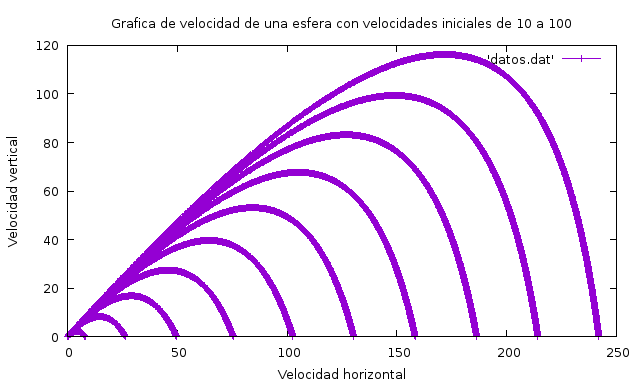
\includegraphics[width=\linewidth]{Resistencia.png}
  \caption{Grafica de posición.}
  \label{fig:boat1}
\end{figure}

\end{document}
